\chapter{研究现状和相关工作}

\section{本章引言}

本章首先介绍了多摄像头系统的发展现状以及发展趋势,并列举了若干多摄像头系统的性能以及实现方法。然后介绍了多摄像头系统同步控制的几种方法,主要可以分为硬件控制和软件控制两大类。最后介绍了对摄像头拍摄时间进行检测的相关方法。

\section{多摄像头系统}

多摄像头系统一般由多个单一摄像头组合形成,包括数据采集,控制,数据存储分析等几部分组成。多摄像头系统的优势在于融合了各个摄像头的优点,并且利用数量上的优势成倍将这些优点放大。如果需要实现多种拍摄要求,就需要摄像头满足多种性能指标,对于单一摄像头来说大多数情况下很难满足,而能够满足要求的摄像头往往较为昂贵或难以获得,甚至有些情况下对于摄像头的多种性能要求是相互矛盾的,根本无法实现,而多摄像头系统就能够很好地解决这一问题。多摄像头系统可以选取多个具有不同性能指标的摄像头,选取所需的功能进行融合即可满足要求。同时还可以利用多个摄像头的融合使其性能指标成倍增长,从而利用廉价摄像头实现了高品质摄像头的功能。

目前多摄像头系统主要可分为两种类型,一类是大规模同类摄像头集成,一类是异种摄像头组合搭配。同类摄像头集成一般采用较多的相同性能参数摄像头组成摄像头阵列,以形成规模优势。Stanford大学计算图形学实验室搭建了一个多摄像头阵列 \cite{3},就是利用了低成本摄像头的价格优势和高性能处理器的运算优势,将100个CMOS图像传感器数码摄像头组成阵列形式。每个摄像头由两部分组成,一部分负责图像采集,由互补金属氧化物半导体(CMOS)图像传感器和廉价镜头组成,一部分负责数据处理,由视频编码器,现场可编程逻辑门阵列(FPGA)和IEEE 1394(Firewire)传输接口组成。该多摄像头系统能够对100个摄像头拍摄到的视频进行实时同步压缩,并将数据保存在硬盘中。

\begin{figure}[h] 
  \centering
  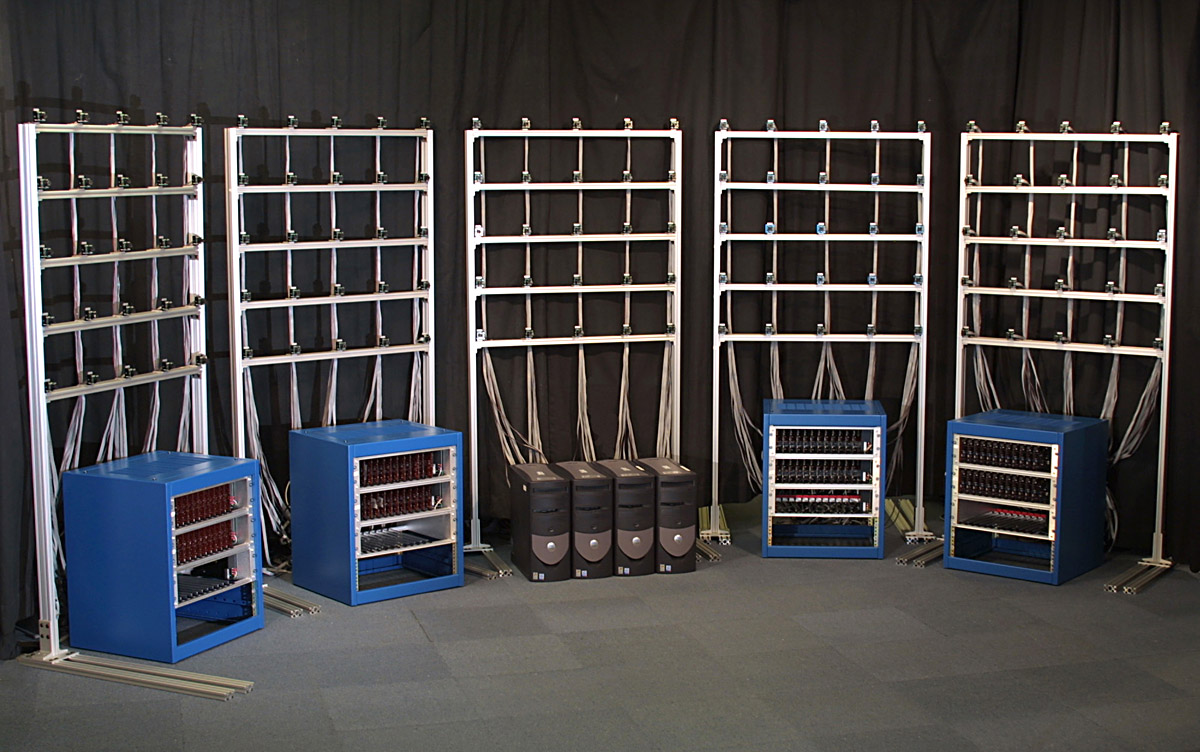
\includegraphics[height=5cm, width=8cm]{Stanford2}
  \caption{Stanford大学多摄像头阵列}
  \label{Stanford2}
\end{figure}

根据各个摄像头排列方式和拍摄角度的不同,该多摄像头系统能够实现多种功能。当各个摄像头紧密排列时,可以将系统视为一个单中心的合成相机,将各个摄像头拍摄到的数据进行合成处理后,就能够大幅度提升各项性能参数,如动态范围、景深、帧率和光谱灵敏度等 \cite{4, 7}。当各个摄像头排列间隔较远时,可以将该系统视为多中心摄像头,即为视场相机。通过该视场相机可以提出新的三维场景重建方法以及多视角全景构建方法 \cite{5}。当各个摄像头间隔排列时,可以将系统视为一个具有大合成孔径相机,这使得该系统可以通过部分闭塞的环境观察拍摄对象,即实现共聚焦镜头的离散近似,其中不在选定平面上的物体变得模糊和黑暗 \cite{6, 8}。

另一类多摄像头系统由不同性能的摄像头组合而成,这样可以充分发挥各个摄像头的性能优势,从而满足使用者对于系统的多种需求。例如在欧洲航天局(ESA)和俄罗斯联邦航天局合作推动的火星探测计划(ExoMars)中 \cite{9, 10},为了能够使火星登陆车实现周边地形勘测,火星车自身定位,大气及周边环境监测,科学实验观测等功能,研究人员将配置在火星车上的全景摄像头(Panoramic Camera)设计成了一个多摄像头系统。该系统是由一个高分辨率摄像头(HRC)和两个广角立体摄像头(WAC)组成。其中高分辨率摄像头的有效像素为1024 × 1024,主要负责细节图像的拍摄。而广角立体摄像头配备视角为65°的镜头,通过两个摄像头采集到的图像进行融合,模拟人家实现立体成像,主要负责观测周围环境。这样,该系统通过不同性能指标的摄像头之间的配合,实现了所需的全部功能。

\begin{figure}[h] 
  \centering
  \includegraphics[height=5cm, width=8cm]{Mars}
  \caption{火星登陆上的全景摄像头}
  \label{Mars}
\end{figure}

目前针对多摄像头系统的研究,多围绕对视频内容的分析展开。例如针对视频内的运动物体进行追踪,在安防监控等领域有较多应用。Ting-Hsun Chang等人在文献 \cite{11} 中提出了一种基于贝叶斯模态融合的方法,利用多摄像头系统追踪室内环境下多个人的移动轨迹。为了连续追踪运动物体,该系统为每个新检测到的对象设定特有的模式,当对象移动或进入到其他摄像头视野内时,系统会利用贝叶斯网络组合匹配各个模式,以实现连续追踪。不同于其他单一摄像头的闭塞推理追踪方法,该方法利用多摄像头系统进行交互追踪,能够大大提高追踪精度。同样Kim等人在文献 \cite{12} 中也提出了一种基于平面跟踪对应模型(TCM)的方法来对大规模多摄像头系统内的对象进行跟踪。该方法为每个运动对象计算了一个唯一且不变的追踪对应模型,使得在不同摄像头的视野内,或者在各个摄像头重叠的视野内,对应同一个物体来说有且只有一个追踪对应模型,这样就能能够准确追踪对象的运动。

还比如针对拍摄图像进行多摄像头校准,以实现更好的拍摄效果。Strecha等人在文献 \cite{13} 中为了实现基于图像的三维建模技术,需要将各个摄像头进行校准并实现多角度立体视觉。Baker等人在文献 \cite{14} 中为了校准各个摄像头,利用LED灯光建立点对(point correspondences),输入到大规模非线性特征值最小化程序当中,使得各个摄像头两两之间建立全息投影矩阵。Kurillo等人在文献 \cite{15} 中提出了一种广域校准方法,利用LED灯光标识作为校准对象,利用矩阵分解计算摄像头初始姿态,并通过自动构建加权视觉图,同时在相机之间找到最佳的变换路径来解决全局校准。

另外一些研究是针对多摄像头拍摄结果进行拼接。Hongming Zhang等人在文献 \cite{16} 中为了解决前景对象在视频拼接过程中造成的割裂问题,提出了一种前景对象边缘调整的方法。该方法将各个摄像头拍摄到的图像进行前景提取,并根据前景图像的内容动态调整拼接边缘,再对于静态的背景图像进行拼接,最后将前景图像与背景图像进行融合即可得到拼接结果。

\section{多摄像头系统的同步控制}

多摄像头系统的同步控制,其主要的目的是为了能够精确控制系统内各个摄像头的拍摄时间,以减小拍摄时间误差对拍摄结果造成的影响。例如,当利用多个摄像头从不同角度拍摄某一对象时,如果该对象静止不动,则各个摄像头的拍摄时间存在误差也不会影响拍摄结果。但是如果该对象是在不断变化,则各个摄像头会在不同时刻拍摄到该对象的不同状态,如果各个摄像头之间并非精确同步,其拍摄时间存在一定波动,那么就无法拍摄到同一时刻该对象的相同状态。同样,当利用多个摄像头按照一定的时间间隔,在不同时刻连续拍摄某一对象的变化,如果各个摄像头之间并非时间同步,那么就无法控制其按照设定好的时间间隔拍摄,可能会发生拍摄时间的重叠、提前或延后。

现阶段,对多摄像头系统进行同步控制,主要分为硬件控制和软件控制两种。利用硬件进行控制时,需要通过特殊的硬件接口,如IEEE-1394接口、Camera Link接口等,将系统内各个摄像头连接到一起,通过控制器发送控制信号给摄像头。而利用软件进行控制----------

\subsection{硬件同步}

硬件同步控制主要可分为两类:一类是利用多路图像数据采集卡实现,一类是利用外部触发信号源实现。

图像数据采集卡是一种对摄像头图像数据进行获取、处理、存储等功能的硬件设备。通过硬件接口同摄像头进行连接,接口的种类包括模拟接口,如AV接口、S端子等,和数字接口,如PCI总线、USB接口等。图像数据采集卡一般都集成了对摄像头的控制模块、编解码模块、存储模块等功能模块,因此具有多个输出接口的采集卡能够对多路摄像头进行控制。在图像数据采集卡的使用过程当中,一般对于摄像头的要求较高,需要摄像头具有专门的通信接口能够同采集卡进行连接,并且能够对采集卡的输出信号进行相应,同时也要保证采集到的数据能够被采集卡所识别。虽然采用图像数据采集卡能够在硬件层面对多路摄像头进行比较精确的同步控制,但是由于此类采集卡多为成熟产品,开放性较低,难于对其进行更底层地控制,同时对于摄像头的要求限制也较多。

目前市面上可以购买的图像数据采集卡种类很多,其主要差别在于摄像头接口种类,输出路数以及其他一些附加功能。同样也有很多研究关于设计并实现多路图像数据采集卡。如朱海宽等人在文献 \cite{17} 中设计并实现了一种基于PCI总线的多路图像采集卡;刘晓军等人在文献 \cite{刘晓军2009采用} 中实现了一种具有HD-SDI高清串行数字接口的FPGA视频采集卡;王剑飞等人在文献 \cite{王剑非2007基于} 中实现了在Linux平台下的视频采集设备的驱动程序。

为了消除图像数据采集卡在使用过程中的种种限制,更多的多摄像头系统采用外部触发信号源实现同步控制功能。这类系统内的各个摄像头都具有触发信号的收发接口,通过接口与控制器相连接,控制器根据系统需求在特定的时刻发送触发信号给各个摄像头。姜广文等人在文献 \cite{姜广文} 中提出了一种基于外触发的多摄像头同步系统的设计方法。该方法采用USB接口的数字输出模块作为同步触发信号发生器,将高精度的触发信号发送给各个摄像头,实现同步功能。国蓉等人在文献 \cite{国蓉2014具有} 中利用同步信号发生器和锁相环电路实现同步功能。当摄像头接收到同步触发信号后,开始进行曝光拍摄,经试验验证,触发信号与摄像头拍摄周期之间的相位差为10\textmu s

\subsection{软件同步}


\section{摄像头拍摄时间检测}



\section{本章小结}










































